\documentclass{article}

\usepackage{graphicx}
\usepackage{tikz}
\usepackage{tikzsymbols}
\usetikzlibrary{calc,patterns,shapes.geometric}
\pagestyle{empty}
\usepackage[margin=0pt]{geometry}
\geometry{papersize={14in,12in}}

\def\centerarc[#1](#2)(#3:#4:#5){\draw[#1] ($(#2)+({#5*cos(#3)},{#5*sin(#3)})$) arc (#3:#4:#5);}

\begin{document}
	\begin{figure}
		\centering
		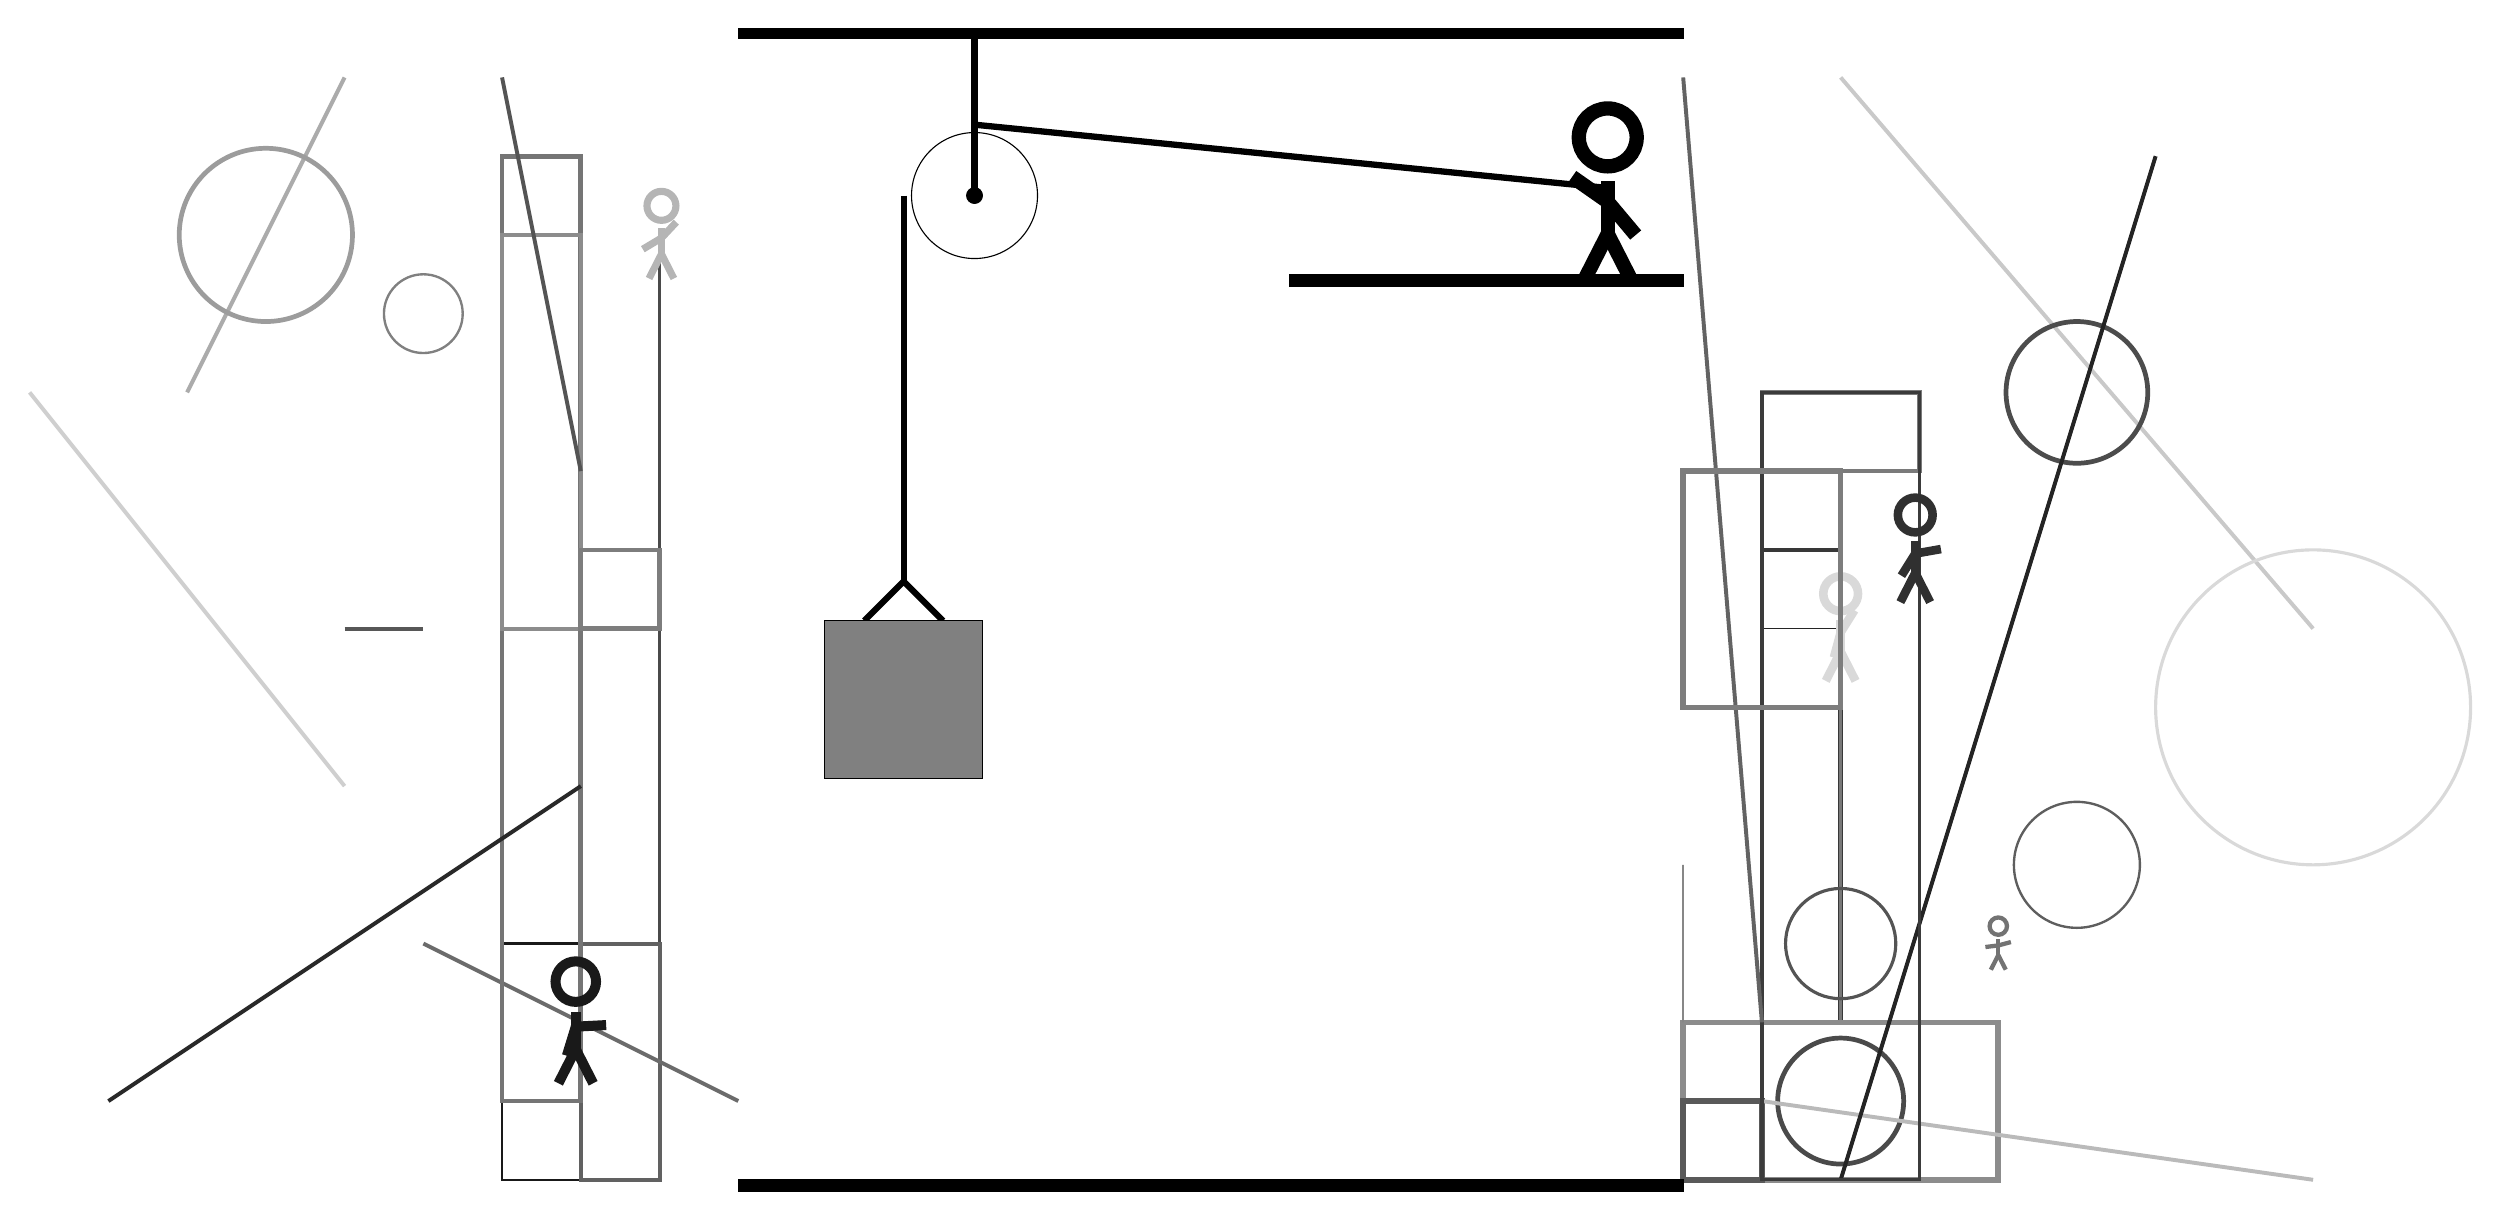
\begin{tikzpicture}
			%%%%% START %%%%%
			
			\draw[fill=black] (-2, 11.5) rectangle (10, 11.625);
			
			\draw (1, 9.5) circle (0.8);
			\draw[fill=black] (1, 9.5) circle (0.1);
			\draw[line width=0.8mm] (1, 11.5) -- (1, 9.5);
			
			\draw[line width=0.3mm, color=black!90] (-3, -3) rectangle (-5, 0);
			
			\draw [line width=0.6mm, color=black!71](12, -2) circle (0.8);
			\draw[line width=0.5mm, color=black!21](12, 11) -- (18, 4);
			\draw[line width=0.6mm, color=black!78] (11, 5) rectangle (12, -1);
			\draw[line width=0.3mm, color=black!53] (12, 3) rectangle (12, -1);
			
			\draw[line width=0.3mm, color=black!71] (-3, 9) rectangle (-3, -2);
			\draw [line width=0.3mm, color=black!63](15, 1) circle (0.8);
			\draw[line width=0.5mm, color=black!62] (-4, 0) rectangle (-3, -3);
			\node[line width=0.3mm, color=black!55] at (14, 0) {\Strichmaxerl[3][7][15]};
			\draw[line width=0.7mm, color=black!45] (10, -1) rectangle (14, -3);
			\draw[line width=0.2mm, color=black!86] (11, 4) rectangle (12, 4);
			\draw[line width=0.5mm, color=black!58](-6, 0) -- (-2, -2);
			\draw[line width=0.3mm, color=black!47] (10, 1) rectangle (10, -1);
			\draw[line width=0.5mm, color=black!33](-7, 11) -- (-9, 7);
			\draw [line width=0.6mm, color=black!39](-8, 9) circle (1.1);
			\draw [line width=0.4mm, color=black!15](18, 3) circle (2.0);
			
			\draw [line width=0.3mm, color=black!50](-6, 8) circle (0.5);
			
			\draw[line width=0.7mm, color=black!65] (10, -3) rectangle (11, -2);
			\draw[line width=0.5mm, color=black!27](11, -2) -- (18, -3);
			
			\draw[line width=0.6mm, color=black!54] (-4, -2) rectangle (-5, 10);
			\draw[line width=0.6mm, color=black!52] (11, 7) rectangle (13, 6);
			
			\draw[line width=0.5mm, color=black!84](-4, 2) -- (-10, -2);
			\draw[line width=0.5mm, color=black!45] (-4, 9) rectangle (-5, 4);
			\draw[line width=0.6mm, color=black!51] (-3, 4) rectangle (-4, 5);
			\draw [line width=0.6mm, color=black!70](15, 7) circle (0.9);
			\draw[line width=0.5mm, color=black!66](-7, 4) -- (-6, 4);
			
			\node[line width=0.6mm, color=black!15] at (12, 4) {\Strichmaxerl[6][75][58]};
			\draw[line width=0.5mm, color=black!86](12, -3) -- (16, 10);
			\draw[line width=0.4mm, color=black!77] (11, -3) rectangle (13, 7);
			
			\draw[line width=0.5mm, color=black!67](-4, 6) -- (-5, 11);
			\draw[line width=0.5mm, color=black!61](11, -1) -- (10, 11);
			
			\draw[line width=0.7mm, color=black!51] (12, 6) rectangle (10, 3);
			\node[line width=0.2mm, color=black!90] at (-4, -1) {\Strichmaxerl[7][73][3]};
			
			\draw[line width=0.5mm, color=black!19](-7, 2) -- (-11, 7);
			
			\node[line width=0.2mm, color=black!81] at (13, 5) {\Strichmaxerl[6][58][10]};
			\draw [line width=0.4mm, color=black!67](12, 0) circle (0.7);
			\node[line width=0.7mm, color=black!29] at (-3, 9) {\Strichmaxerl[5][31][47]};
			
			\draw[line width=0.8mm](-0.4, 4.1) --  (0.1, 4.6) -- (0.6, 4.1);
			\draw[fill=black!50] (-0.9, 4.1) rectangle (1.1, 2.1);
			
			\draw[line width=0.8mm](0.1, 9.5) -- (0.1, 4.6);
			\centerarc[line width=0.8mm](1, 9.5)(90:180:0.9)
			\draw[line width=0.8mm](1, 10.4) -- (9, 9.6);
			
			\node at (9, 9.5) {\Strichmaxerl[10][-35][-50]};
			\draw[fill=black] (5, 8.5) rectangle (10, 8.35);
			
			\draw[fill=black] (-2, -3) rectangle (10, -3.15);
			
			%%%%% END %%%%%
		\end{tikzpicture}
	\end{figure}	
\end{document}